% prelim.tex -- owner: merging task.  Section owners: request changes through NOTES.md.
% Drawn from KATKA Sections 2 and 5 and More RLBWT Tricks Section 2.
\section{Preliminaries}
\label{sec:prelim}

\subparagraph*{Strings.}
We index strings from $0$.
For a string $Y$, $Y[i..j]$ is the substring from position $i$ to position $j$ inclusive, $Y[i..j)$ is $Y[i..j - 1]$, and $Y[i..]$ is the suffix starting at position $i$.
Each section defines its own text $T[0..n)$, which ends with a sentinel \texttt{\$} that occurs nowhere else and is smaller than every other character.
A pattern, which in Sections~\ref{sec:zymo} and~\ref{sec:silva} is a read, is called $P$.
We find matches over $\{\texttt{A},\texttt{C},\texttt{G},\texttt{T}\}$ only: patterns are split at other characters, such as runs of~\texttt{N}, and $T$ is built so that no match crosses a separator.

\subparagraph*{BWTs.}
The suffix array $\mathrm{SA}$ lists the starting positions of the suffixes of $T$ in lexicographic order, the BWT~\cite{BurrowsWheeler1994} is $\mathrm{BWT}[i] = T[(\mathrm{SA}[i] - 1) \bmod n]$, and we call $i$ a \emph{row}.
For a string $X$, $\intv(X)$ is the (possibly empty) interval of rows whose suffixes start with $X$, the \emph{BWT interval} of $X$.
LF maps the row of a suffix to the row of the suffix one character longer, $\Psi = \mathrm{LF}^{-1}$, so that $\mathrm{SA}[\Psi(i)] = \mathrm{SA}[i] + 1$, and $\phi$ maps $\mathrm{SA}[i]$ to $\mathrm{SA}[i - 1]$.
A \emph{backward step} computes $\intv(cX)$ from $\intv(X)$ for a character $c$, and \emph{backward search}~\cite{FerraginaManzini2000} for $P$ applies backward steps for the characters of $P$ from right to left.
We use it to find the longest suffix of a string that occurs in $T$, with its interval.
For strings $X \ne Y$ of the same length, $\intv(X)$ and $\intv(Y)$ are disjoint; and LF preserves the order of rows with equal BWT characters, so the rows of $\intv(X)$ whose suffixes are preceded by a string $\alpha$ are mapped one-to-one and in order onto $\intv(\alpha X)$.

\subparagraph*{RLBWTs and RLCSAs.}
Let $r$ be the number of maximal runs of equal characters in the BWT.
For a highly repetitive text, such as a collection of genomes of one species, $r$ is small, and indexes built on the run-length compressed BWT (RLBWT), such as the RLFM-index~\cite{MakinenNavarro2005}, the RLCSA~\cite{MakinenEtAl2010} and the r-index~\cite{GagieNavarroPrezza2020}, take space proportional to~$r$~\cite{Navarro2021}.
We use two kinds.
Our \emph{RLBWT}, as in an RLFM-index, stores the run starts in Elias--Fano coded bitvectors~\cite{OkanoharaSadakane2007} and the run characters in a wavelet tree, and a backward step is two rank queries, whose cost grows with the size of the alphabet.
Our \emph{RLCSA}, in the form of Brown et al.~\cite{BrownEtAlRLCSA}, stores for each character $c$ the sorted list of the starting rows of the runs of $c$ in the BWT, with the cumulative lengths of those runs, so that a backward step by $c$ is a predecessor search in the list of $c$, whose cost does not depend on the size of the alphabet; the lists are either plain arrays (an \emph{explicit} RLCSA) or Elias--Fano coded.
Both give the same intervals.
Sections~\ref{sec:zymo} and~\ref{sec:silva} index DNA with an explicit RLCSA, since the tag array of Section~\ref{sec:tags} needs no access to the BWT itself and the RLCSA is faster; Section~\ref{sec:chr19} indexes DNA with an RLBWT, which it also uses to map between levels, and stores the BWTs of a parse and of a sequence of blocks, whose alphabets have millions of symbols, like an RLCSA.

\subparagraph*{Both strands and the reversed collection.}
Finding a MEM needs extensions to the right as well as to the left, and backward search extends only to the left.
There are two standard ways around this, and we use both.
In Sections~\ref{sec:zymo} and~\ref{sec:silva}, $T$ contains every sequence and its reverse complement (reversed, with \texttt{A} and \texttt{T}, and \texttt{C} and \texttt{G}, swapped), so a read matches $T$ whichever strand it came from, and extending a match to the right by a base $c$ is the same as extending its reverse complement to the left by the complement of $c$; backward search alone then extends matches in both directions, although switching direction means searching again for the reverse complement of the whole match.
In Section~\ref{sec:chr19}, $T = S_1 \# S_2 \# \cdots S_d \# \$$ is a collection of genomes, on the forward strand only, and we also index the \emph{reversed collection} $T' = S_d^{\mathrm{rev}} \# \cdots S_1^{\mathrm{rev}} \# \$$: a string without separators occurs in $T$ if and only if its reverse occurs in $T'$, so a backward search over the RLBWT of $T'$ for the reverse of $P[x..]$ finds the largest $e$ such that $P[x..e)$ occurs in $T$.

\subparagraph*{MEMs.}
A \emph{maximal exact match} (MEM) of $P$ is a substring $P[a..e)$ that occurs in $T$ while $P[a - 1..e)$ (if $a > 0$) and $P[a..e + 1)$ (if $e < |P|$) do not.
Maximality is thus with respect to intervals of the pattern, not to pairs of occurrences as is usual in stringology, and these MEMs are the super-maximal exact matches (SMEMs) of Li~\cite{Li2012} and of Tagger~\cite{DAF+25}.
We usually want only the MEMs of length at least a threshold~$L$.
\emph{Forward--backward search}~\cite{Li2012} finds all the MEMs: it alternates a forward search from a position $x$, which gives the largest $e$ such that $P[x..e)$ occurs, with a backward search from $e$, which gives a MEM $P[a..e)$ and its interval, and a backward search from $e + 1$, which gives the next starting point $x$.

\subparagraph*{Boyer--Moore--Li.}
BML~\cite{Gagie2024BML,Li2024} finds the MEMs of $P$ of length at least $L$.
Starting with $x = 0$, it checks whether a MEM of length at least $L$ starts in $P[x..]$ by searching backward for the window $P[x..x + L)$, starting from its right end.
If the step that prepends $P[j - 1]$ fails, so that $P[j - 1..x + L)$ does not occur, then no MEM of length at least $L$ starts at a position from $x$ to $j - 1$, and BML jumps to $x = j$, skipping the rest of the window as in Boyer--Moore pattern matching.
If the whole window occurs, BML extends the match to the left as far as it can, to some position $a$, then to the right, with a forward search from $a$, to some position $e$, reports the MEM $P[a..e)$ and continues with $x = e - L + 1$, the first window that ends after the MEM.
\Cref{fig:bml} shows an example.
Gagie~\cite{Gagie2024BML} gives the theory, the full version~\cite{Gag24arxiv} gives a practical algorithm, and Li implemented BML in ropebwt3~\cite{Li2024}.
On an index of both strands, the forward extension ends with the BWT interval of the MEM's reverse complement, whose occurrences are in the same taxa as the MEM's, which is all Sections~\ref{sec:zymo} and~\ref{sec:silva} need.
BML and forward--backward search use only searches for the longest suffix of a substring of $P$ that occurs in $T$ (or in $T'$, or as a reverse complement), so any method that returns the same longest suffix and interval as backward search can be plugged into them without changing their output~\cite{Gagie2024BML}; Section~\ref{sec:chr19} relies on this.

\begin{figure}[t]
\centering
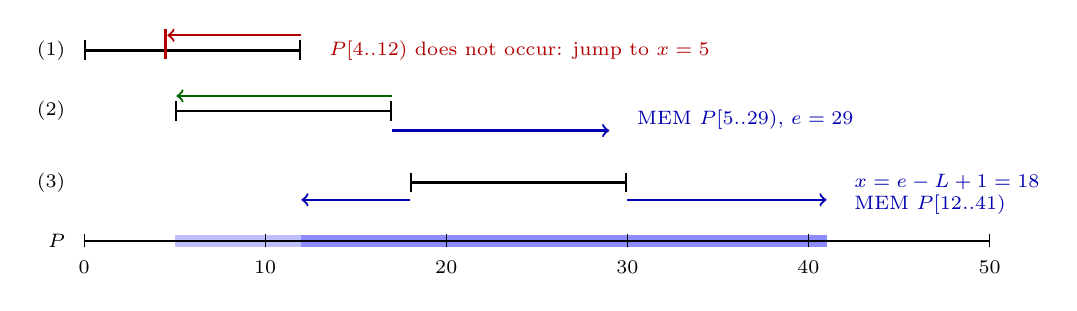
\begin{tikzpicture}[x=2.3mm, y=5.5mm, every node/.style={font=\scriptsize}]
\fill[blue!25] (5,-0.13) rectangle (29,0.13);
\fill[blue!45] (12,-0.13) rectangle (41,0.13);
\draw[thick] (0,0) -- (50,0); \node[anchor=east] at (-0.5,0) {$P$};
\foreach \i in {0,10,20,30,40,50} { \draw (\i,-0.15) -- (\i,0.15); \node[below=2pt] at (\i,-0.1) {\i}; }
\node[anchor=east] at (-0.5,4.4) {(1)};
\draw[|-|, thick] (0,4.4) -- (12,4.4);
\draw[->, red!70!black, thick] (12,4.75) -- (4.6,4.75); \draw[red!70!black, thick] (4.5,4.2) -- (4.5,4.9);
\node[red!70!black, anchor=west] at (13,4.4) {$P[4..12)$ does not occur: jump to $x = 5$};
\node[anchor=east] at (-0.5,3.0) {(2)};
\draw[|-|, thick] (5,3.0) -- (17,3.0);
\draw[->, green!40!black, thick] (17,3.35) -- (5.1,3.35);
\draw[->, blue!70!black, thick] (17,2.55) -- (29,2.55);
\node[blue!70!black, anchor=west] at (30,2.8) {MEM $P[5..29)$, $e = 29$};
\node[anchor=east] at (-0.5,1.35) {(3)};
\draw[|-|, thick] (18,1.35) -- (30,1.35);
\draw[->, blue!70!black, thick] (18,0.95) -- (12,0.95);
\draw[->, blue!70!black, thick] (30,0.95) -- (41,0.95);
\node[blue!70!black, anchor=west] at (42,1.35) {$x = e - L + 1 = 18$};
\node[blue!70!black, anchor=west] at (42,0.85) {MEM $P[12..41)$};
\end{tikzpicture}
\caption{Boyer--Moore--Li with $L = 12$ on a pattern $P$.
(1)~The search for the window $P[0..12)$ fails at the step that prepends $P[4]$, so no MEM of length at least $L$ starts at positions 0 to 4, and BML jumps to $x = 5$.
(2)~The window $P[5..17)$ occurs; it cannot be extended to the left, since $P[4..17)$ contains $P[4..12)$, so BML extends it to the right and reports the MEM $P[5..29)$.
(3)~The next window is $P[18..30)$; BML extends it in both directions, to the MEM $P[12..41)$, and continues with $x = 30$.}
\label{fig:bml}
\end{figure}

\subparagraph*{Longest MEMs.}
BML can also find the longest MEMs of a pattern in one pass, without a threshold: start with $L = 1$ and, whenever a MEM longer than $L$ is found, set $L$ to its length.
Raising $L$ only stops the search for MEMs shorter than one already found, and a MEM as long as the current $L$ is still found, so the longest MEMs, including ties, are among those reported; as $L$ grows, BML skips more of the pattern.
We call this \emph{BML with adaptive $L$}.
The experimental appendix of the full version of Gagie's BML paper~\cite{Gag24arxiv} already found a longest MEM this way, keeping $L$ one more than the length of the longest MEM found so far; keeping $L$ equal to that length also reports ties.

\subparagraph*{KeBaB.}
KeBaB~\cite{BrownEtAl2025KeBaB} first cuts a pattern into \emph{pseudo-MEMs}, the maximal substrings of length at least $k$ all of whose $k$-mers pass a Bloom filter of the $k$-mers of $T$, so that every MEM of length at least $k$ lies in a pseudo-MEM and only the pseudo-MEMs need to be searched.
